\documentclass[11pt]{amsart}
\usepackage{geometry}                % See geometry.pdf to learn the layout options. There are lots.
\geometry{letterpaper}                   % ... or a4paper or a5paper or ... 
%\geometry{landscape}                % Activate for for rotated page geometry
%\usepackage[parfill]{parskip}    % Activate to begin paragraphs with an empty line rather than an indent
\usepackage{graphicx}
\usepackage{amssymb}
\usepackage{lscape}

\usepackage{epstopdf}
\usepackage{verbatim}
\usepackage{rotating}
\usepackage{multirow}
\usepackage{multicol}
\usepackage{booktabs}
\usepackage{subfigure}

\usepackage{algorithm}
\usepackage{algpseudocode}
\DeclareGraphicsRule{.tif}{png}{.png}{`convert #1 `dirname #1`/`basename #1 .tif`.png}
\newtheorem{proposition}{Proposition}
\newtheorem{definition}{Definition}
\newcommand{\vertgeq}{\rotatebox{90}{$\leq$}}

\title{Draft}
\author{Lapo Santi}
%\date{}                                           % Activate to display a given date or no date

\begin{document}
\maketitle
%\section{}
%\subsection{}
\tableofcontents

\newpage

\section{Introduction}
Introduction:

The purpose of this paper is to introduce a novel methodology to infer the latent ordering of blocks that exhibit a transitivity property in directed networks. Specifically, we develop a method to infer the community structure of binary interactions, where the groups are ordered in a one-dimensional hierarchy that determines the preferred edge direction. The paper builds on a class of models closely related to stochastic blockmodels, where only non-negative entries are considered. However, in this model, we are ignoring the zero entries, which can be debatable whether we are still dealing with a network as we are ignoring the sparsity that is one of the staples of networks.

Research Question:

The research question of this paper is to infer the block structure underlying a set of binary interactions with transitivity properties in directed networks. Our approach advances the existing literature by considering a method to learn the ordering of the blocks that reflects better an ordering of the block themselves.

Importance of the Study:

This paper innovates the field of statistics by providing a novel methodology to infer the latent ordering of blocks, which can be very useful under certain circumstances. The proposed method has practical applications in analyzing tennis tournament data, where we can learn how competitive a tournament is by inferring the blocks and their ordering, from the strongest to the weakest.

Objectives:

The objective of this paper is to develop a method to infer the community structure of binary interactions where the groups are ordered in a one-dimensional hierarchy that determines the preferred edge direction. Specifically, we aim to learn the ordering of the blocks that exhibit a transitivity property in directed networks.

Methodology:

We start by introducing the theory behind Partially Ordered Markov Models (POMMs) and the definition of a Strong Stochastic Transitivity matrix (SST matrix). Then we combine the two ideas into one, showing that we can represent the SST matrix with a collection of level sets. We impose a very specific dependence structure between the blocks, a Markovian one. Next, we specify the full model, where outcomes of tennis matches are represented as a binomial distribution, the POMM ordering is imposed on the entries of the winning probability matrix, and a dirichlet multinomial distribution is imposed on the assignment of players to blocks. This distribution is expanded into a Chinese Restaurant Process (CRP), which can be used to avoid assumptions on the initial number of blocks. Initially, we assume that the number of blocks follows a Poisson distribution. Finally, we simulate data and test our methodology with simulated data, followed by applying it to a real tennis dataset.

Outline of the Paper:

This paper is organized as follows. Section 2 introduces the theory behind Partially Ordered Markov Models (POMMs) and the definition of a Strong Stochastic Transitivity matrix (SST matrix). In Section 3, we combine the two ideas into one, showing that we can represent the SST matrix with a collection of level sets. Section 4 describes the dependence structure imposed on the blocks, a Markovian one, and how we specify the full model. In Section 5, we explain how we expand the dirichlet multinomial distribution into a Chinese Restaurant Process (CRP) and the assumptions we make on the number of blocks. Section 6 presents our simulation study, where we test our methodology with simulated data. Finally, in Section 7, we apply our methodology to a real tennis dataset. We conclude the paper with a discussion of our findings and potential future research directions.




\newpage
\section{Posets and Dags}
\begin{definition}\label{def:Poset}[Poset]To define poset, a partially ordered set we start from $D$, a set of elements. The binary relation $\prec$ on $D$ is said to be a partial order if:
\begin{align}
&\text{For any } x \in D, x \prec x (\text{ reflexivity }) \\
&\text{For any } x,y,z \in D, x \prec y \text{ and } y \prec z \implies x \prec z (\text{ transitivity }) \\
&\text{For any } x, y \in D, x \prec y \text{ and } y \prec x \implies x = y (\text{ antisymmetry }).
\end{align}
Then we call $(D, \prec)$ a partially ordered set, or a \textit{poset}. 
\end{definition}

A \textit{finite poset} $(D,\prec)$ is a poset where $D$ has a finite number of distinct elements. 

Example: let $D$ be the finite set defined by representing the $M \times N$ array of probabilities. Let $(u,v)$ and (q,r) be any two elements of $D$ and define the binary relation on $D$ by
\begin{equation}
(q,r) \prec (u,v) \iff q \prec u \text{ and } r \prec v
\end{equation}

There exists a correspondence between posets and directed cyclic graphs. 

Let $(D, F)$ be a directed acyclic graph, where $D = \{y_1, \ldots, y_n\}$, a finite set. To construct a poset to which this digraph corresponds, we define the binary relation $\prec$ on D by
\begin{align}
&y_i \prec y_i \text{ for } i= 1\dots n \\ 
&y_i \prec y_j \text{ if there exists a directed path from } y_i \text{ to } y_j \in (D,F)
\end{align}

We saw above that the correspondence is many-to-one. Given a finite poset, one may construct a class of directed acyclic graphs; the correspondence described above is in a sense the minimal directed acyclic graph since it has the smallest possible directed edge set
Pomms definitions 


\begin{definition}[Cone]
For any $y \in D$, the \textit{cone} of $y$ is the set
\begin{equation}
\text{ cone } y = \{x \in D: x\prec y;x\neq y \} \nonumber
\end{equation}
\end{definition}

\begin{definition}[Adjl]
For any $y \in D$ the \textit{adjacent lower neighbourhood} of $y$ is the set $$
\text{adjl } y = \{ x \in D:(x,y) \text{is a directed edge in} (D,F)\}
$$
\end{definition}

\begin{definition}[Dilation]
For any $y \in D$, the \textit{dilation} of $y$ is the set 
\begin{equation}
\text{dil } y = \bigcup\{ \overline{\text{adjl }} x : y \in \overline{\text{adjl }} \} \nonumber
\end{equation}
\end{definition}

\begin{definition}[Excluded dilation]
For any $y \in D$, the \textit{excluded dilation}  of $y$ is the set 
\begin{equation}
\text{dil }^* y = \text{dil } y \setminus \{y\}
\end{equation}
\end{definition}

\begin{definition}[Minimal element]
In general, an element $y\in D$ is called \textit{minimal element} if there is no other element $x$ satisfying $x\prec y$ where $\text{ adjl } s$ is the set of adjacent lower neighbors of $s \in D$.
\end{definition}


\begin{definition}[Cover of a Subset]
The cover of a subset $B$ is a set of all elements $x$ in $D$ such that $x$ is adjacent to an element in $B$ and $x$ is not in $B$. Formally, the cover of $B$ is defined as follows:
\begin{equation}
\text{covr}\ B = { x \in D: \text{adjl}\ x \subset B \text{ and } x \notin B } \nonumber
\end{equation}
where $\text{adjl}\ x$ is the set of all adjacent elements of $x$ in $D$.
\end{definition}
Intuitively, the cover of a subset $B$ represents all the elements in $D$ that are outside of $B$ but are adjacent to at least one element in $B$. In other words, the cover of $B$ captures the neighborhood of $B$ in $D$.

\begin{definition}[Level Sets]
The level sets of a poset $D$ are a sequence of nonempty cover sets defined recursively as follows:
\begin{equation}
L^0 = D_{min};\quad L^i = \text{covr}\left( \bigcup_{k=0}^{i-1} L^k \right) \nonumber
\end{equation}
where $D_{min}$ is the set of all minimal elements in $D$.
\end{definition}

The first level set $L^0$ is simply the set of all minimal elements in $D$. The subsequent level sets are defined by taking the union of all the previous level sets and taking the cover of this union. Intuitively, each level set captures the neighborhood of the previous level sets in $D$.



\subsection{Partially ordered Markov models:}

Consider a finite set of random variables $\{ Z(s_1),\ldots,Z(s_n) \}$ indexed by location or "points" $$
D = \{s_1,\ldots ,s_n \}: n \in \{1,2,\ldots \}
$$

That is, we assume the existence of a directed acyclic graph $(D,F)$ and its corresponding poset $(D,\prec).$
Let $(D,F)$ be a finite, directed acyclic graph and its corresponding poset $(D,\prec).$ Consider $s \in D$ and recall the definition of cone $s$. Also, let the quantity $U_s$ denote any subsets of points not related to s. 
Formally:
$$
U_s \subset \{ u \in D: u \text{ and } s \text{ are not related } \}
$$
\begin{definition}[POMM]
Then $\{ Z(s): s \in D \}$ is said to be a partially ordered Markov model (POMM) if , for all $s \in D$ and any $U_s$
\begin{equation}
P(Z(s)|Z(\text{ cone } s), Z(U_s)) = P(Z(s)|Z(\text{ adjl } s)
\end{equation}
\end{definition}
\begin{proposition}\label{eq:result1}[Joint Distribution]
Let $(D,F)$ be a directed acyclic graph with no singleton points and let $(D, \prec)$, be its associated poset. Suppose that $\{Z(s): s \in D\}$ is a POMM. Then 
\begin{align}
P(Z(D)) &= P(Z(L^0)) \prod_{k=1}^m \prod \{ P(Z(u))| Z(\text{ adjl } u): u \in L^k \} \\
&= P(Z(L^0)) \prod \{ P(Z(u))| Z(\text{ adjl } u): u \in D 
\setminus L^0 \}
\end{align}
where $L^0, L^1, \ldots L^m$ are the level sets as defined previously.
\end{proposition}







Result 1 relates the probability of a random variable defined on a poset to the probabilities of its restrictions to the lower level sets of the poset.

The result states that the probability of $Z$ on the entire poset $D$ can be expressed as a product of the probabilities of $Z$ restricted to the level sets $L^0, L^1, \ldots, L^m$ of the poset, where $L^0 = D_{\text{min}}$ is the set of minimal elements of $D$, and $L^k$ is the set of elements of $D$ that are not in any of the previous level sets $L^0, L^1, \ldots, L^{k-1}$ and whose immediate predecessors are all in the union of the previous level sets $\bigcup_{i=0}^{k-1} L^i$.

The first part of the result states that the probability of $Z$ on $D$ is equal to the product of the probability of $Z$ on $L^0$ and the conditional probabilities of $Z$ on the elements of each subsequent level set $L^k$, given the values of $Z$ on their immediate predecessors. This can be seen as a form of the chain rule of probability, where the joint probability of $Z$ on $D$ is decomposed into a product of conditional probabilities.

The second part of the result simplifies the product by noting that the conditional probabilities of $Z$ on the elements of $D\setminus L^0$ are determined by the values of $Z$ on their immediate predecessors, which are all in $L^0$ or $D\setminus L^0$. Therefore, the product can be simplified to the product of the probability of $Z$ on $L^0$ and the conditional probabilities of $Z$ on the elements of $D\setminus L^0$ given the values of $Z$ on their immediate predecessors in $D\setminus L^0$. This simplification reduces the number of terms in the product and makes the computation of the joint probability of $Z$ on $D$ more efficient.




\newpage







\section{Application to the SST matrix}



In this section, I will introduce a matrix that displays the Strong Stochastic Transitivity (SST) property. The aim of this section is to model the probability of a player winning a match in a tournament against another one. To achieve this goal, we need to ensure that the probabilities are arranged in a consistent manner. Specifically, we want to ensure that if Player A is stronger than Player B, and Player B is stronger than Player C, then Player A must be stronger than Player C. This is a well-known mathematical concept known as transitivity, and it is essential to impose it on the probabilities of victory between the players. For instance, if we know that Djoković is stronger than Medvedev and Medvedev is stronger than Kyrgios, then we can infer that Djoković must be stronger than Kyrgios. By using the SST property, we can guarantee that the probabilities of victory reflect this logical relationship, which enhances the clarity and coherence of our model.
After having introduced the SST property, we want to build upon the definitions of Section(1), and re-express the SST matrix within the POMMs' framework. This new definition will allow us to have a coherent and tractable framework to express the joint probability distribution of such ordered probabilities and, ultimately, to perform inference.

\subsection{Defining matrix P (SST matrix)}
The matrix under consideration, that is $P$, is a collection of victory probabilities among $K$ entities, which could represent players or also groups of players. The matrix is denoted by $\underset{K \times K}{P}$, where $K$ is the number of players/ group of players taken into consideration. 

\begin{center}
$$P = 
\left(\begin{array}{cccc}p_{1,1} & p_{1,2} &  ... & p_{1,K} \\ p_{2,1} & p_{2,2} & ... & p_{2,K} \\ \vdots & \vdots & \vdots & \vdots \\ p_{K,1}& p_{K,2 }& ... & p_{K,K}\end{array}\right)$$
\end{center}



Each element $p_{i,j}$ in the matrix $P$ represents the probability of player $i$ winning over player $j$ in a tennis match, where draws are not permitted. Therefore, it must be the case that $p_{i,j} + p_{j,i} = 1$ in order to satisfy the requirements for a valid probability. It follows that $p_{j,i}$ can be expressed as $1 - p_{i,j}$. The lower triangular entries of matrix $P$ can be determined from the upper triangular entries. Consequently, our focus is on modelling the upper triangular part of $P$.
 
Without loss of generality, we can assume that player/team 1 is the strongest, and player/team $K$ is the weakest.

From this assumption, it follows that the elements in the upper triangular part of the matrix must remain above $0.5$ to maintain the assumption of monotonicity in the probabilities. Violation of this assumption could lead to a contradiction where a weaker player/team has a higher probability of winning than a stronger one. For instance, if $p_{1,2} = 0.4 \leq 0.5$, then $p_{2,1} = 0.6$ would imply that player 1 is weaker than player 2, which is contradictory with our baseline assumption. Furthermore, we set the main diagonal of matrix $P$ to $0.5$ for teams and $0$ for individual players.

Therefore, we must constrain the probabilities as follows:

\begin{itemize}
\item The probabilities must increase monotonically as the index of the columns $j$ increases;
\item The probabilities must decrease monotonically as the index of the rows $i$ increases.
\end{itemize}
The matrix $P$ with the described modification will look like this: 
\begin{center}
$$
\left(\begin{array}{ccccccc} 0.5 & \leq & p_{1,2} & \leq &  ... & \leq & p_{1,K} \\  &  & \vertgeq &  & ... &  & \vertgeq \\
1 - p_{1,2} & \leq & 0.5 & \leq & ... & \leq & p_{2,K} \\ \vdots & \vdots & \vdots & \vdots &  ... & \vdots& \vdots \\ 1 - p_{1,K}& \leq & 1 - p_{2,K}& \leq & ... & \leq & 0.5\end{array}\right)
$$
\end{center}


\begin{figure}
\begin{center}
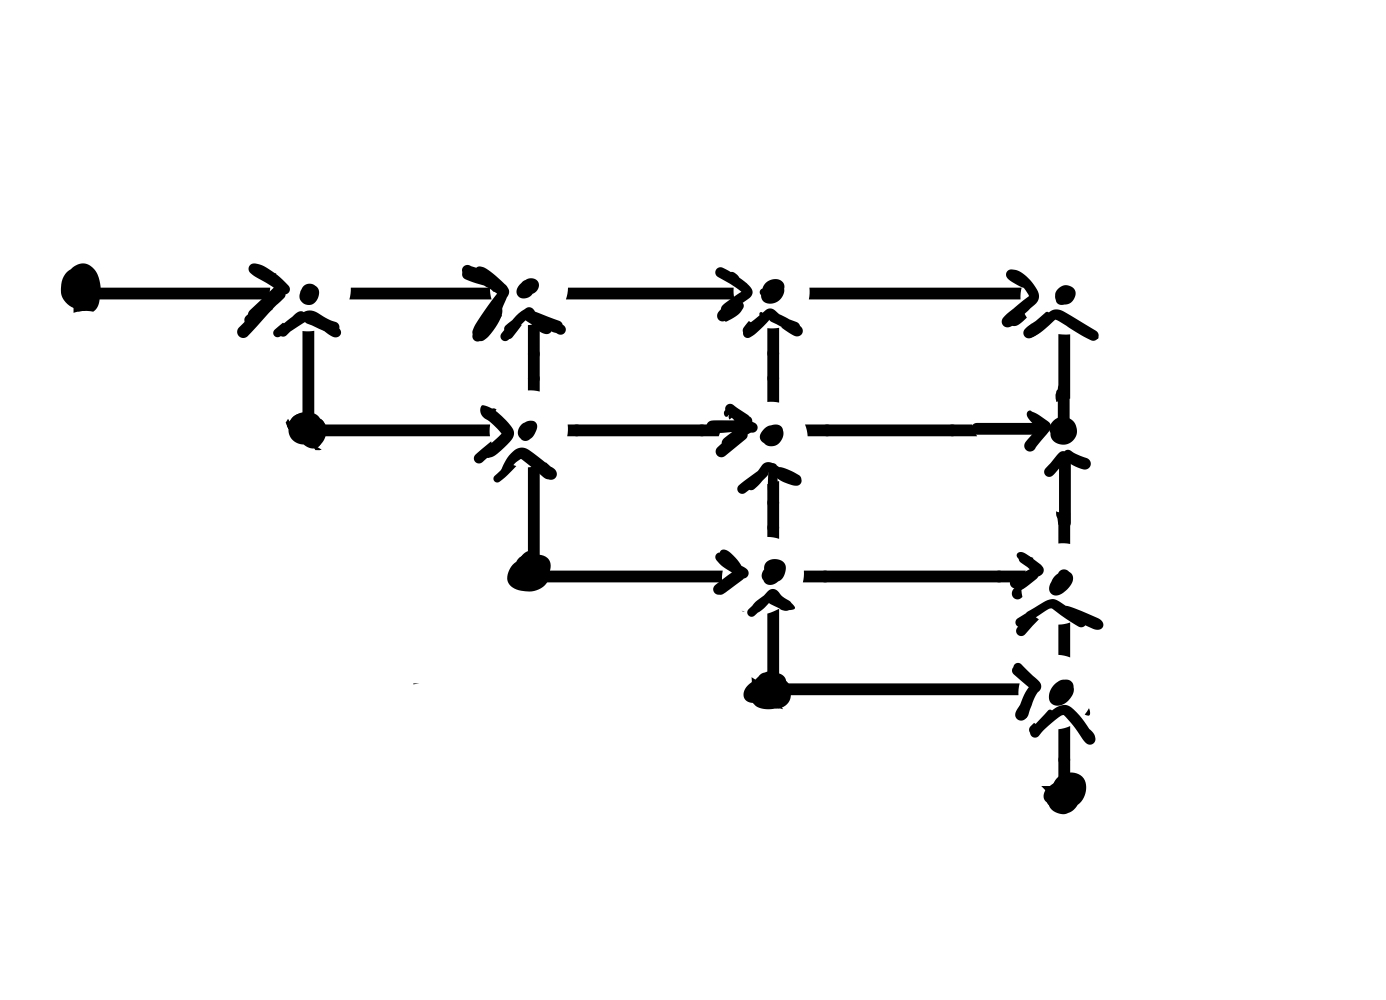
\includegraphics[width=0.6\textwidth,natwidth=1386,natheight=1000]{/Users/lapo_santi/Desktop/Nial/project/POMMs/IMG_0EE4E8AB347D-1.jpeg}
\caption{Dag representation of the Poset imposed onto the SST matrix}
\label{fig:DAG}
\end{center}
\end{figure}

\subsection{Defining a Poset over $P$}
Having defined $P$, now we want to re-define it within a finite Poset framework to obtain $(P, \leq)$. Let $(i,j)$ and $(p,q)$ be two elements of $P$ and define the binary relation $\leq$ on $P$ as 
\begin{equation}
(p,q) \leq (i,j)  \iff p \leq i \text{ and } q \leq j
\end{equation}

Now, $(P, \leq)$ is clearly a Poset since it satisfies the three properties of Definition \eqref{def:Poset}. We represent the corresponding directed acyclic graph $(P,F)$, where $F$ is the set of directed edges between vertices in Figure (\ref{fig:DAG}) by using the definition of Adjacent Lower Neighborhood that we introduced before.



\begin{definition}[Cone over $P$]In this case, for any $(i,j) \in D$ the cone of $(i,j)$ is the set:
\begin{equation}
\text{cone } (i,j)  = \{(i,j-1), \ldots (i,i), (i+1,j), \dots,(K,j) \}
\end{equation}
\end{definition}
\begin{definition}[$\overline{\text{cone }} (i,j)$]
In this case, for any $(i,j) \in P$ the closure of the cone of $(i,j)$ is the set:
\begin{equation}
\overline{\text{cone }} (i,j)  = \{(i,j), \ldots (i,i), (i,j), \dots,(K,j) \}
\end{equation}
\end{definition}

\begin{definition}[The adjacent lower neighborhood of $(i,j)$]
In this case, for any $(i,j) \in P$ the adjacent lower neighborhood of $(i,j)$ is the set:
\begin{equation}
\text{adjl } (i,j)  = \{(i,j-i), (i+1,j)\}
\end{equation}
\end{definition}

\begin{definition}[closure of $\text{adjl } (i,j)$]
In this case, for any $(i,j) \in P$ the closure of $\text{adjl } (i,j)$ is the set:
\begin{equation}
\overline{\text{adjl }} (i,j)  = \{(i,j-i), (i+1,j), (i,j)\}
\end{equation}
\end{definition}

\begin{definition}[$D_{min}^P$]
In this case, the \textit{minimal element} denoted by $D_{min}$ is such that
\begin{equation}
P_{min}  = \{(i,j) \in P: i=j\}
\end{equation}
namely the main diagonal of the $P$ matrix. 
\end{definition}
\begin{figure}
\begin{center}
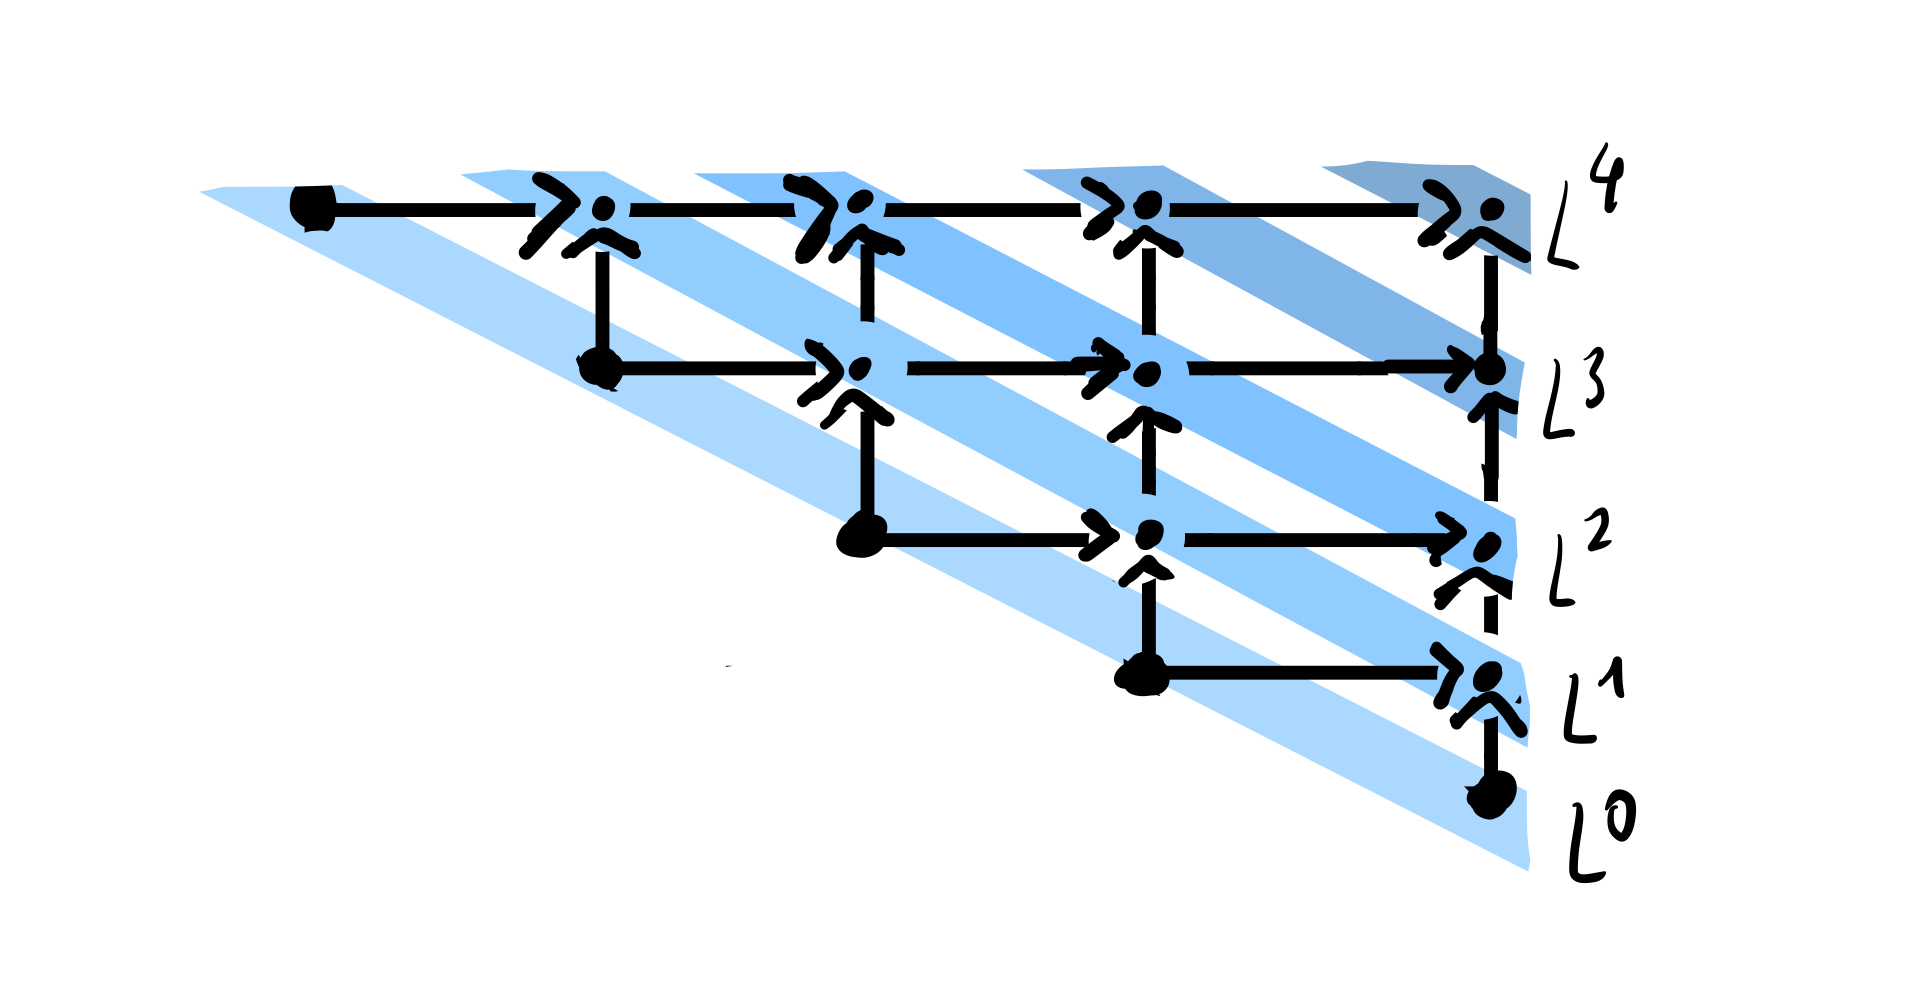
\includegraphics[width=0.6\textwidth,natwidth=1921,natheight=1000]{/Users/lapo_santi/Desktop/Nial/project/POMMs/level_sets.jpeg}
\caption{Visual Display of the level sets $L^k: k=0,\ldots,4$}
\label{fig:level_sets}
\end{center}
\end{figure}


The \textit{level sets} of $P$, in this case, corresponds to the diagonals above the main one.


\subsection{Partially ordered Markov Models applied to P}
\bigskip
Considering the finite set of random variables $\{P_{1,1},\dots, P_{K,K} \}$ indexed by locations where 
$$D\equiv \{(1,1), \dots (K,K)\}$$

Having showed the existence of a directly acyclic graph $ (P,F)$ and its corresponding poset $(P, \leq)$, we can write down 
\begin{align}
P(P_{ij}| Z(\text{cone } i,j)) &= P(P_{ij}| P(\text{adl } i,j))\\
P(P_{ij}| P_{i+1,j}, P_{i,j-1})
\end{align}

Now, exploiting Proposition \eqref{eq:result1}, we can write:
\begin{equation}
P(P(D)) = \prod_{i=1}^K\prod_{j=i}^K P(P_{ij}| P_{i+1,j}, P_{i,j-1})
\end{equation}


\begin{comment}
\section{Truncated specifications: hard constraint}

The modeling choice is a truncated beta distribution. The truncation helps us in various respects:
\begin{enumerate}
\item \textit{Parsimony}: The truncation in correspondence of the maximum value of the two adjacent lower neighbors of a given entry $p_{i,j}$ gives us the possibilityof obtaining the result SST property with just one parameter, namely the variance of the beta.
\item \textit{Stability}: The beta parameters' space is less regular than one might think. First, when one expresses $\alpha, \beta$ in terms of expected value $\mu$ and variance $\sigma^2$ we need to bear in mind that $\sigma^2 < \mu(1-\mu)$ to have $ \alpha, \beta > 0 $. A second problematic aspect is that if the prior process reaches the value $p_{i,j}^{(s)} = 1$ for some values $i,j$, the subsequent value will be not defined because the support of a beta distributed variable is $[0,1]$, but by the constraint of the process itself $p_{i,j}^ {(s+1)}> 1$, which is not defined. For this reason, it is necessary to truncate to $\approx .9999$ each variable of the process.
\item \textit{Consistency}: The truncation at $M$ ensures that $100\%$ of the sampled matrices will respect the desired SST property.
\end{enumerate}






\subsection{Truncated Beta Distribution with fixed variance}
$$P(p_{i,j}|\text{adjl}(p_{i,j})) = \text{Beta}\left(\alpha, \beta; 0, \mathbb{I}(p_{ij} \geq \max_{z \in \text{adjl}(p_{i,j})} z)\right)$$
where $\text{Beta}(\alpha, \beta)$ denotes the beta distribution with parameters $\alpha$ and $\beta$, and $1(\max_{z \in \text{adjl}(p_{i,j})} z)$ is the truncation at the maximum of the adjacent lower neighbourhood, from now on denoted by M.  The parameters $\alpha$ and $\beta$ are set such that:
\begin{align}
\mathbb{E}[p_{i,j}|\text{adjl}(p_{i,j})] &= M\\
Var[p_{i,j}|\text{adjl}(p_{i,j})] &= \lambda
\end{align}

\subsection{Truncated Beta Distribution with variance varying with column and row index}
$$P(p_{i,j}|\text{adjl}(p_{i,j})) = \text{Beta}\left(\alpha, \beta; 0, \mathbb{I}(p_{ij} \geq M_z)\right)$$ where $\text{Beta}(\alpha, \beta)$ denotes the beta distribution with parameters $\alpha$ and $\beta$, and $1(\max_{z \in \text{adjl}(p_{i,j})} z)$ is the truncation at the maximum of the adjacent lower neighborhood, from now on denoted by M.  The parameters $\alpha$ and $\beta$ are set such that:
\begin{align}
\mathbb{E}[p_{i,j}|\text{adjl}(p_{i,j})] &= M \\
Var[p_{i,j}|\text{adjl}(p_{i,j})] &= \lambda * (j-i)
\end{align}

where $(j-i)$ is increasing as we get closer to the upper-right corner. The following matrix containing the values is an example:
\begin{table}
\begin{center}\begin{tabular}{cccc}0 & 1 & 2 & 3 \\-1 & 0 & 1 & 2 \\-2 & -1 & 0 & 1 \\-3 & -2 & -1 & -0\end{tabular} \caption{A $4\times4$ matrix where the element $A_{i,j} = (j-i)$}
\end{center}
\label{defaulttable}
\end{table}


\subsection{Truncated Beta Distribution with variance specified for each $(ij)$}



$$P(p_{i,j}|\text{adjl}(p_{i,j})) = \text{Beta}\left(\alpha, \beta; 0, \mathbb{I}(p_{ij} \geq M_z)\right)$$

where $\text{Beta}(\alpha, \beta)$ denotes the beta distribution with parameters $\alpha$ and $\beta$, and $1(\max_{z \in \text{adjl}(p_{i,j})} z)$ is the truncation at the maximum of the adjacent lower neighbourhood, from now on denoted by M.  The parameters $\alpha$ and $\beta$ are set such that:
\begin{align}
\mathbb{E}[p_{i,j}|\text{adjl}(p_{i,j})] &= M\\
Var[p_{i,j}|\text{adjl}(p_{i,j})] &= \lambda_{ij}
\end{align}
where $\lambda_{ij}$ is varying across the elements, guaranteeing maximal flexibility but possibly creating identifiability issues.






\end{comment}





















\newpage


\begin{comment}
\section{Stick-Breaking prior process}

In this section, we define a generative process for the SST matrix using the POMM framework. We consider the above-defined level sets $L^1, \ldots, L^K$ for a $K-$ dimensional matrix $P$ and we specify a hyperprior distribution process over the POMM one. In particular, we will resort to a modified version of the stick-breaking prior process to create matrices which satisfy the SST property. 


\subsection{General definition of the Stick-Breaking prior process}
\bigskip
A Stick-Breaking prior process, conceptually, involves repeatedly breaking off and discarding a random fraction (sampled from a Beta distribution) of a "stick" that is by default of length 1. 
The distribution drawn is discrete with probability 1. In the stick-breaking process view, we explicitly use the discreteness and give the probability mass function of this (random) discrete distribution as:

$$ f(\theta) = \sum_{k=1}^{\infty} \beta_k \cdot \delta_{\theta_k}(\theta) $$

where $\delta_{\theta_k}$ is the indicator function which evaluates to zero everywhere, except for $\delta_{\theta_k}(\theta_k)=1$. Since this distribution is random itself, its mass function is parameterized by two sets of random variables: the locations $\left\{\theta_k\right\}_{k=1}^{\infty}$ and the corresponding probabilities $\left\{\beta_k\right\}_{k=1}^\infty $. 

The probabilities $\beta_k$ are given by a procedure resembling the breaking of a unit-length stick (hence the name).
\begin{equation}
\beta_k = \beta^{\prime}_k\cdot\prod_{i=1}^{k-1}\left(1-\beta^{\prime}_i \right)
\end{equation}

where $\beta^{\prime}_k $are independent random variables with the beta distribution $\operatorname{Beta}(1,c)$. The resemblance to 'stick-breaking' can be seen by considering $\beta_k$ as the length of a piece of a stick. We start with a unit-length stick and in each step, we break off a portion of the remaining stick according to $\beta^{\prime}_k$ and assign this broken-off piece to $\beta_k$. The formula can be understood by noting that after the first $k-1$ values have their portions assigned, the length of the remainder of the stick is $\prod_{i=1}^{k-1}\left(1-\beta^{\prime}_i\right)$ and this piece is broken according to $\beta^{\prime}_k$> and gets assigned to $\beta_k$

The smaller $c$ is, the less of the stick will be left for subsequent values (on average), yielding more concentrated distributions. 



\subsection{Application to the SST case}

In the context of the specific case, the level sets of the POMM are defined as the locations $\theta_k$, and a stick-breaking prior is imposed on them through truncated Beta distributions. The first step is to define the $\operatorname{Beta}(1,c)$ distributed random variables, namely  $b^i$: we do that in Equation \eqref{eq:beta_dist}. Then, $p_i$ values are generated according to the stick-breking process as in Equation \eqref{eq:stick_breaking}. The step in equation \eqref{eq:mapping} maps these proportions from the $[0,1]$ interval to the $[0.5, \beta^0_{\max}]$ one, via the function $f^{\beta^0_{\max}}$, which is nothing but a linear transformation of the values. Moreover, since we want to induce an increasing behaviour in the boundaries for the $p_{ij}$ we take the cumulative sum of the simulated $p_i$. Finally, in Equation \eqref{eq:truncation} we simulate the entries of the POMM from a $\operatorname{Beta}(1,1)$, where we have different truncations depending on the level set, meaning those entries $\{p_{ij} \in P :(j-i) = k\} \quad \text{ for } k = 1, \ldots, K $.

Here is the full model specification of a $\operatorname{POMM}(c,\beta^0_{\max},K)$ process:

\begin{align}
b_i &\sim \operatorname{Beta}(1,c) \quad &\text{ for } i = 1,\ldots,K \label{eq:beta_dist}\\
p_i &\sim b_i \prod_{j=1}^{i-1} (1 - b_j) \quad &\text{ for } i = 1,\ldots,K \label{eq:stick_breaking}\\
\beta^0_i &= f_{[0,1]\rightarrow[0.5, \beta^0_{\max}]} \left( \sum_{j=1}^i p_j \right) \quad &\text{ for } i = 1,\ldots,K \label{eq:mapping}\\
p_{ij} &\sim \operatorname{Beta}(1,1) \mathbb{I}(\beta^0_{k-1} <L^k < \beta^0_{k+i} ) \quad &\text{ for } (j-i) = k, \quad \text{ for } k= 1,\ldots,K \label{eq:truncation}
\end{align}

where $c$ is the concentration parameter, $\beta^0_1 = 0.5$ and $\beta^0_{\max}$ is the maximum value that the entries $p_{ij}$ can take.

To investigate the role of $c$, we have represented in Figure \ref{fig:cvalues} the evolution of the process $\beta^0_i \quad \text{ for } i = 1,..., K$ according to different $c$ values. We have done the same for the hyper-parameter $\beta^0_{\max}$ in Figure \ref{fig:differentbetavalues}. Finally, the resulting stick-breaking prior can be visualized in Figure \ref{fig:POMMpriormatrix} an example of the simulated matrix given $K=10,c=3,\beta^0_{\max} = .7$.

The overall joint probability distribution is as follows:
\begin{align}
p(p_{ij} \in P|c,\beta^0_{\max})&= \prod_{k=1}^K \prod_{ij: (j-i)=k}^{((K-1)*K)/2} \frac{1}{\operatorname{Beta}(1,1)}\mathbb{I}(\beta^0_{k-1} < L^k < \beta^0_{k+i}) \\
 &\times \prod_{k=1}^K \left(\beta_k^0 \right)^{-1} \prod_{j=1}^{k-1} (1 - \left(\beta_j^0\right)^{-1}) \\ 
 &\times\prod_{k=1}^K \frac{1}{\operatorname{Beta}(1,c)} b_k (1-b_k)^{c-1}
\end{align}

where $\left(\beta_k^0\right)^{-1}= f_{[0.5, \beta^0_{\max}]\rightarrow [0,1]} \left( \Delta_{j=1}^{k} \beta_j^0 \right) $ where $\Delta$ computes the cumulative difference of the boundaries for the truncated beta distribution. 

In practice, we are first mapping back the observed truncation from $[0.5, \beta^0_{\max}]$ to the space $[0,1]$, and then take the inverse of the cumulative summation in \eqref{eq:mapping} using the $\Delta$ operator. 


Overall, the Stick-Breaking prior process provides a rigorous and coherent method for generating discrete distributions with a flexible and controllable parametrization 



\begin{figure}[htbp]
    \centering
    \begin{minipage}{.5\textwidth}
        \centering
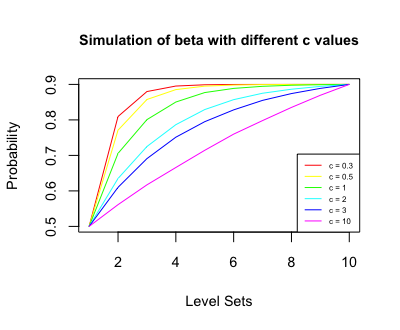
\includegraphics[width=\textwidth,natwidth=400,natheight=330]{/Users/lapo_santi/Desktop/Nial/project/POMMs/Stick-Breaking prior/Differentcvalues.png}
\caption{The plot shows the evolution of the $\beta^0$ prior process for different $c$ values and $\beta^0_{\max} = 0.9 $. Every line corresponds to a different concentration parameter $c$, as shown in the legend.}
\label{fig:cvalues}
\end{minipage}\hfill
    \begin{minipage}{.5\textwidth}
        \centering
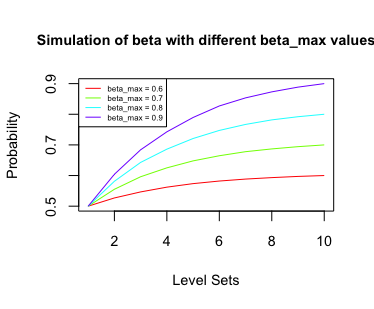
\includegraphics[width=\textwidth,natwidth=374,natheight=309]{/Users/lapo_santi/Desktop/Nial/project/POMMs/Stick-Breaking prior/differentbetavalues.png}
\caption{The plot shows the evolution of different $\beta^0$ prior processes. Every line corresponds to a different $\beta_{max}$ value, given a concentration parameter $c = 3$. }
\label{fig:differentbetavalues}
\end{minipage}
\hfill
    \begin{minipage}{\textwidth}
        \centering
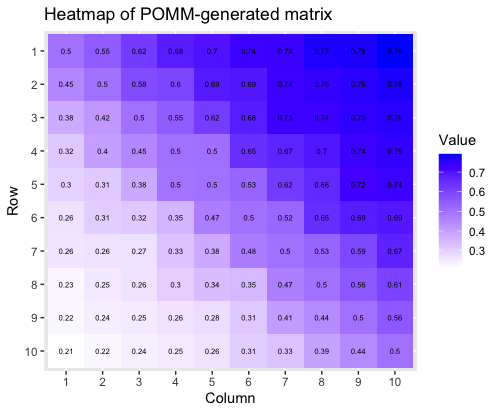
\includegraphics[width=0.5\textwidth,natwidth=500,natheight=413]{/Users/lapo_santi/Desktop/Nial/project/POMMs/Stick-Breaking prior/Heatmap_pomm.png}
\caption{The plot shows a POMM matrix generated with parameters $K=10,c=3,\beta_{max} = 0.8$. The higher value is 0.79, which means that we are able to enforce the truncation as wanted. The parameter $c=3$ translates into a moderately concentrated matrix, where we do not have big differences in players' winning probability}
\label{fig:POMMpriormatrix}
\end{minipage}
 \end{figure}




\end{comment}





\newpage

\section{Power Law prior process}

The Power Law process is used to generate a prior process that can produce a SST matrix with a desired degree of flexibility. The probability values in the SST matrix should increase in the columns and decrease in the rows. To achieve this effect, the Power Law process uses level sets, which correspond to the diagonals in the upper triangular part of the matrix. The entries within each level set are modelled as truncated beta distributions with parameters (1,1).

More specifically, let us denote the set of upper triangular entries of the matrix as $U = {(i,j) \in \mathbb{N}^2 : i \leq j}$. Then, we can use the notation $\mathbf{P}_{(i,j) \in U}$ to represent the upper triangular entries of the matrix $\mathbf{P}$. The probability density function of the entries in the upper triangular part of the matrix can be written as:

\begin{equation}
p(\mathbf{P}{(i,j) \in U}) = \prod{k=1}^K \prod_{j-i=k}^{|L^{(k)}|} \frac{1}{y^{(k+1)} - y^{(k)}} = \prod_{k=1}^K \left( \frac{1}{y^{(k+1)} - y^{(k)}} \right)^{|L^{(k)}|}
\end{equation}

where $|L^{(k)}|$ is the cardinality of the level set $L^{(k)}$, and $y^{(k)}$ is the truncation point of the beta distribution that corresponds to level set $k$.

The truncation generating process starts with the function $f(x) = x^\alpha + 0.5 \in [0.5, \beta^0_{\max}]$, which is a monotonically increasing function that is linear for $\alpha = 1$, concave for $\alpha \in (0,1)$, and convex for $\alpha > 1$. The function is used to provide truncation points for the beta distributions.

To generate truncations, we take the inverse function of $f(x)$, denoted as $f(y)^{\leftarrow} = (y - 0.5)^{(1/\alpha)}$. The support of $f(x)$ is then found to be $[f(0.5)^{\leftarrow}, f(\beta^0_{\max})^{\leftarrow}] = [0, (\beta^0_{\max} - 0.5)^{(1/\alpha)}]$, which is then divided into $K$ segments of equal length $\Delta = ((\beta^0_{\max} - 0.5)^{(1/\alpha)} - 0) / K$. The segment endpoints are defined as $x_k = \Delta \times (k-1)$ for $k=1,\ldots,K+1$. The cumulative sum of the segment endpoints is then mapped back to $f(x)$, resulting in $K$ truncation points $y^{(k)}$, which are defined as:

\begin{equation}
y^{(k)} = f(x_k) = \left( \frac{(\beta^0_{\max} - 0.5)^{(1/\alpha)}}{K} \times (k-1) \right)^\alpha + 0.5
\end{equation}


\subsection{Specific case: main diagonal equal to 0.5}






Let us define once again $Y = L(\alpha)^k$. Then let us denote with $p^Y$ the pdf of $Y$ and with $p^\alpha$ the pdf of $\alpha$. We have that:
\begin{align}
\label{eq:pdfy}
p_Y(y^{(k)}|\mu, \sigma^2) &= \left| \frac{d L^{-1}(y^{(k)})}{d(y^{(k)})} \right| \cdot p^\alpha \left( L^{-1}(y^{(k)}) \right) \\
&= \left| \dfrac{2}{\ln\left(\frac{(k-1)}{K-1}\right)\left(2y^{(k)}-1\right)} \right| 
 \frac{1}{\sqrt{2\pi\sigma^2}} \exp{\left( -\frac{1}{2\sigma^2}  \left( \frac{\ln \left( y^{(k)} - 0.5 \right) -  \ln \left(  (\beta^0_{\max} - 0.5) \right)}{ \ln \left( \frac{(k-1)}{K-1} \right) }- \mu \right)^2 \right) } \nonumber \\
 & \mathbb{I}\left(\frac{\ln \left( y - 0.5 \right) -  \ln \left(  (\beta^0_{\max} - 0.5) \right)}{\ln \left( \frac{(k-1)}{K} \right) } > 0 \right) \nonumber
\end{align} 

\begin{comment}
$L$ is a deterministic transformation. Substituting $f(x)$ and $\Delta$ one can find:
\begin{equation}
L^k(\alpha) = \left( \frac{(\beta^0_{\max} - 0.5)^{(1/\alpha)}}{K} \times (k-1) \right)^\alpha  + 0.5
\end{equation}


To find the inverse function of $L(\alpha)^k$, we need to solve for $\alpha$ in terms of $L$. We can start by isolating the term inside the parentheses. To simplify the notation we can set $y:= L(\alpha)^k$.

\begin{align*}
y&= \left( \frac{(\beta^0_{\max} - 0.5)^{(1/\alpha)}}{K} \times (k-1) \right)^\alpha + 0.5 \\
y - 0.5 &= \left( \frac{(\beta^0_{\max} - 0.5)^{(1/\alpha)}}{K} \times (k-1) \right)^\alpha \\
\end{align*}

Next, we can take the logarithm of both sides:

\begin{align*}
\ln \left( y - 0.5 \right) &= \alpha \ln \left( (\beta^0_{\max} - 0.5)^{(1/\alpha)}\times \frac{(k-1)}{K}   \right) \\
\ln \left( y - 0.5 \right) &= \alpha \left[ \frac{1}{\alpha} \ln \left(  (\beta^0_{\max} - 0.5) \right) + \ln \left( \frac{(k-1)}{K}   \right) \right] \\
\ln \left( y - 0.5 \right) &=    \ln \left(  (\beta^0_{\max} - 0.5) \right) + \alpha \ln \left( \frac{(k-1)}{K}   \right) \\
\ln \left( y - 0.5 \right) -  \ln \left(  (\beta^0_{\max} - 0.5) \right) &=    \alpha \ln \left( \frac{(k-1)}{K}   \right) \\
\frac{\ln \left( y - 0.5 \right) -  \ln \left(  (\beta^0_{\max} - 0.5) \right)}{\ln \left( \frac{(k-1)}{K} \right) } &=    \alpha  \\
\end{align*}
Therefore, the inverse function of $L(\alpha)^k$ is:

\begin{equation}
L^{-1}(y) = \frac{\ln \left( y - 0.5 \right) -  \ln \left(  \beta^0_{\max} - 0.5 \right)}{\ln \left( \frac{(k-1)}{K} \right) }
\end{equation}



Now we can take the derivative with respect to $y$:

\begin{equation} 
 \frac{d L^{-1}(y)}{d(y)}  = 
\dfrac{2}{\ln\left(\frac{(k-1)}{K}\right)\left(2y-1\right)}
\end{equation}

\begin{comment}
Now we have all the ingredients to derive the density of $L(\alpha)^k$ by transforming the probability density of $\alpha$, namely $p^\alpha(\alpha) = Normal(\mu,1)\mathbb{I}(\alpha>0)$.

Let us define once again $Y = L(\alpha)^k$. Then let us denote with $p^Y$ the pdf of $Y$ and with $p^\alpha$ the pdf of $\alpha$. We have that:
\begin{align}
\label{eq:pdfy}
p_Y(y^{(k)}|\mu, \sigma^2) &= \left| \frac{d L^{-1}(y^{(k)})}{d(y^{(k)})} \right| \cdot p^\alpha \left( L^{-1}(y^{(k)}) \right) \\
&= \left| \dfrac{2}{\ln\left(\frac{(k-1)}{K-1}\right)\left(2y^{(k)}-1\right)} \right| 
 \frac{1}{\sqrt{2\pi\sigma^2}} \exp{\left( -\frac{1}{2\sigma^2}  \left( \frac{\ln \left( y^{(k)} - 0.5 \right) -  \ln \left(  (\beta^0_{\max} - 0.5) \right)}{ \ln \left( \frac{(k-1)}{K-1} \right) }- \mu \right)^2 \right) } \nonumber \\
 & \mathbb{I}\left(\frac{\ln \left( y - 0.5 \right) -  \ln \left(  (\beta^0_{\max} - 0.5) \right)}{\ln \left( \frac{(k-1)}{K} \right) } > 0 \right) \nonumber
\end{align} 

Therefore the final prior distribution on the $p_{ij}$ will be:
\begin{align}
p(p_{ij}, L^k | \mu) = p(p_{ij}|L^k, \mu) p(L^k | \mu)
\end{align}
where 
\begin{align}
p(L^k | \mu) &\text{ is like in \eqref{eq:pdfy}} \\
p(p_{ij}|L^k, \mu) &= Beta(1,1) \mathbb{I} \left( p_{ij} : j-i= k \in (L^{k-1},L^{k}) \right)
\end{align}




\begin{figure}
\begin{center}
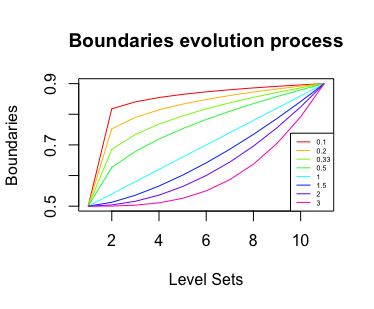
\includegraphics[width=0.6\textwidth,natwidth=374,natheight=309]{/Users/lapo_santi/Desktop/Nial/project/POMMs/power-law prior/boundaryevolution.png}
\caption{ }
\label{ }
\end{center}
\end{figure}
\end{comment}


\begin{figure}[htbp]
    \centering
    \begin{minipage}{\textwidth}
        \centering
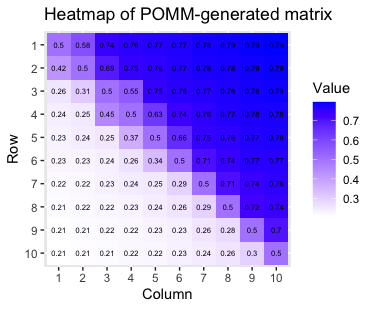
\includegraphics[width=.5\textwidth,natwidth=374,natheight=309]{/Users/lapo_santi/Desktop/Nial/project/POMMs/power-law prior/alpha1_10.png}
        \caption{alpha1\_10.png}
        \label{fig:boxplotnij}
    \end{minipage}\hfill
    \begin{minipage}{\textwidth}
        \centering
        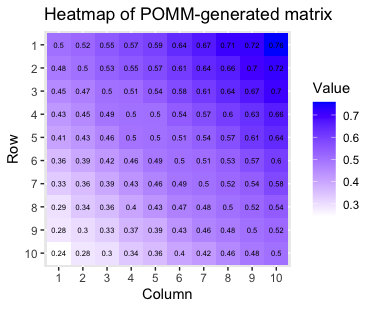
\includegraphics[width=.5\textwidth,natwidth=374,natheight=309]{/Users/lapo_santi/Desktop/Nial/project/POMMs/power-law prior/alpha1.png}
        \caption{alpha1.png}
        \label{fig:densityplotnij}
    \end{minipage}\hfill
    \vskip\floatsep
    \begin{minipage}{\textwidth}
        \centering
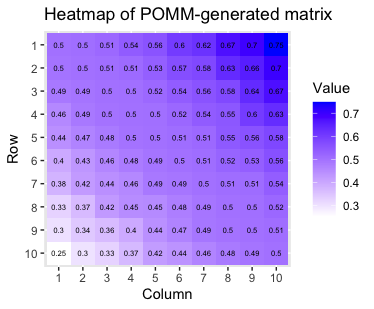
\includegraphics[width=.5\textwidth,natwidth=374,natheight=309]{/Users/lapo_santi/Desktop/Nial/project/POMMs/power-law prior/alpha1_5.png}
        \caption{alpha1\_5.png}
        \label{fig:boxplotyij}
    \end{minipage}
 \end{figure}

\newpage



\section{Full model specification}

The following Bayesian model is used to describe and analyze pairwise data, with the specific aim to identify clusters of points with similar connectivity patterns. 

The model uses a Poisson distribution to model the number of blocks, a Dirichlet-multinomial distribution to model the distribution of nodes' assignment across blocks, and a binomial distribution to model the distribution of edges within blocks. Additionally, the model includes a POMM process to model the probability of edge formation between nodes within blocks.

The goal of the model is to estimate the number of blocks, the distribution of nodes across blocks, and the probability of edge formation between nodes within blocks, given observed network data. The Bayesian approach allows for uncertainty in these estimates and provides a framework for incorporating prior knowledge and updating beliefs as new data becomes available.
\subsection{Model specification}
\bigskip
We denote the nodes in this setting as $1, \dots, n$. We define the model as follows:

\begin{itemize}
\item Let $K$ follow a Poisson distribution $\operatorname{Poisson}(\lambda=1)$, subject to the condition $K>0$.
\item Let $\theta_1, \dots, \theta_K$ be drawn from a Dirichlet distribution with parameter vector $\boldsymbol{\gamma}$.
\item Let $z_i$ be independently and identically drawn from a multinomial distribution with one trial and probability vector $(\theta_1, \dots, \theta_K)$.
\item Let $P = \{p_{i,j}\} \sim \operatorname{POMM}(\alpha,\beta^0_{\max},K)$.
\item Let $y_{i,j}$ follow a binomial distribution with parameters $n_{ij}$ and $p_{z_i, z_j}$, subject to the condition $n_{ij} > 0$.
\end{itemize}

Here, $z_i$ takes values in ${1, \dots, K}$. The likelihood function can be specified as:

\begin{equation}
p(\textbf{y} | p, z) = \prod_{i<j}^{n-1} {n_{ij} \choose y_{ij}} p_{z_i, z_j}^{y_{ij}}(1- p_{z_i, z_j})^{n_{ij}-y_{ij}}
\end{equation}

To specify the prior distribution, we start with the prior on $z$ following a multinomial distribution. We have $n$ players to assign to $K$ different labels, by replacing the extracted labels after each draw. We denote the variable which is the extracted label $i \in \{ 1, ..., K \}$ as $Z_i$, and denote as $\theta_i$ the probability that a given extraction will be of label $i$. The joint probability of $Z_1,\ldots,Z_n$ will be: 
\begin{align}
f(z_1,\ldots,z_n,\theta_1, \ldots, \theta_K ) & {} = \Pr(Z_1 = z_1,\ldots, Z_n = z_n) \\
& {} = \begin{cases} { \displaystyle {n! \over n_1!\cdots n_K!}\theta_1^{n_1}\times\cdots\times \theta_K^{n_K}}, \quad &
\text{when } \sum_{i=1}^K n_i=n \\  \\
0 & \text{otherwise,} \end{cases}
\end{align}

where $n_k = \sum_{i=1}^N \mathbb{I}(z_i = k) \quad \text{ for } k =1,\ldots,K$
for non-negative integers $z_1, ..., z_K$.

The probability mass function can be expressed using the gamma function as:


\begin{equation}
p(z_1, \ldots , z_n| \theta_1, \ldots, \theta_K ) = \frac{\Gamma(\sum_i n_i + 1)}{\prod_i \Gamma(n_i+1)} \prod_{i=1}^K \theta_i^{n_i}
\end{equation}

Here, $n_i$ represents the number of nodes/players allocated to block $i$. On $\theta$, the Dirichlet prior has the following form:

\begin{equation}
f \left(\theta_1,\ldots, \theta_{K}; \gamma_1,\ldots, \gamma_K \right) = \frac{1}{\mathrm{B}(\boldsymbol\gamma)} \prod_{i=1}^K \theta_i^{\gamma_i - 1}
\end{equation}

By marginalizing out $\theta$, following the common practice in the literature, we can express the marginal distribution of $z$ as:
\begin{equation}
p(\textbf{y} | p, z) = \prod_{i<j}^{n-1} {n_{ij} \choose y_{ij}} p_{z_i, z_j}^{y_{ij}}(1- p_{z_i, z_j})^{n_{ij}-y_{ij}}
\end{equation}
\begin{equation} p(\mathbf{z}|\boldsymbol{\gamma}) = \frac{\Gamma(\sum_{i=1}^k \gamma_i)}{\prod_{i=1}^k \Gamma(\gamma_i)}\frac{\prod_{i=1}^k \Gamma(n_i+\gamma_i)}{\Gamma(\sum_{i=1}^k (n_i+\gamma_i))}
\end{equation}

where $\mathbf{z} = (z_1, z_2, \dots, z_k)$ is a vector of labels for $k$ different categories, $\boldsymbol{\gamma} = (\gamma_1, \gamma_2, \dots, \gamma_k)$ is a vector of hyperparameters, and $\Gamma(\cdot)$ is the Gamma function.
For the distribution of $P$ we refer to the previous section in which we have detailed the specification. 

Finally, we specify the prior distribution for the parameter $K$ as:
\begin{equation}
p(K| \lambda =1) = \frac{1^K e^{-1}}{K!} =  \frac{1}{e\cdot K!} \propto \frac{1}{ K!}
\end{equation}

\begin{comment}
\newpage
\section{Simulating synthetic data: code description}


The code \texttt{simulating\_tournament\_test} simulates a tournament with multiple matches between players who belong to different clusters. The number of clusters is simulated from a truncated Poisson distribution, and each player within a cluster is assigned to one of the possible clusters using a Dirichlet multinomial distribution. Then, for each cluster pair, the probability of a player from one cluster winning against a player from another cluster is calculated using POMM process. Finally, a given number of matches between random pairs of players is simulated, where the number of victories of each player is also simulated based on a binomial distribution.

More specifically, the function takes the following arguments:
\begin{itemize}
\item \texttt{n}: the total number of players in the tournament.
\item $\boldsymbol{\gamma}$: a parameter which controls the size of the blocks
\item $c$: a parameter which controls the dispersion of the probabilities within the matrix $P$
\item $\beta_{\max}$: a parameter which controls the probability of victory of the strongest player.
\item \texttt{min\_clust} and \texttt{max\_clust}: the minimum and the maximum number of clusters that can be created using a truncated Poisson distribution.
\item \texttt{M}: the number of matches to be simulated.
\item \texttt{n\_ij\_max}: the maximum number of games that can be played between any two players within the tournament.
\end{itemize}

\subsection{Simulating $K$}\bigskip

As we already said, $K$ is simulated according to a truncated Poisson, i.e., 
\begin{equation} 
K \sim Poisson(\lambda=1) \mathbb{I}(\texttt{min\_clust}< K < \texttt{max\_clust}) 
\end{equation} distribution with parameter. As for \texttt{min\_clust}, \texttt{max\_clust}, they are input under the choice of the user, to better control the number of clusters. In order to sample from the truncated poisson we use inverse sampling:
\begin{align}
U &\gets Unif (0,1) \nonumber \\ 
K &\gets F^{-1}(((F(b, \lambda) - F(a, \lambda))*u+ F(a, \lambda)),\lambda))
\end{align}
where $F$ is the CDF of a Poisson distribution with parameter $\lambda$ and $a,b$ are respectively the lower and the upper truncations. In our specific case we have $\lambda =1, a = \texttt{min\_clust}, \texttt{max\_clust}$
Also in the following parts, when we will need to simulate a truncated Beta distribution, we will use the same method.

\subsection{Simulating $z|K$}\bigskip
After obtaining $K$, each player in the tournament is assigned to a cluster using a Dirichlet multinomial distribution with a concentration parameter denoted by $\boldsymbol{\gamma}$. This is done under the assumption that cluster 1 is the strongest and cluster $K$ is the weakest. The parameter $\boldsymbol{\gamma}$ controls the expected size of the clusters, namely how many nodes are assigned to each label. Three cases are presented to explain the reasoning behind $\boldsymbol{\gamma}$, which are not exhaustive. The three cases are as follows:

\begin{itemize}
\item $\boldsymbol{\gamma} = 1 \quad \forall k \in {1,\ldots,K}$, where the expected size of each cluster is the same.
\item $\boldsymbol{\gamma} = \left[ 1,\ldots, K \right]$, where the expected size of the clusters is inversely proportional to the probability of victory;
\item $\boldsymbol{\gamma} = \left[ K, \dots, 1 \right]$, where the expected size of the clusters is directly proportional to the probability of victory.
\end{itemize}

Given $\boldsymbol{\gamma}$, the probability distribution $p$ is simulated using the gamma distribution:
\begin{equation}
p \gets \texttt{rgamma}(K,\boldsymbol{\gamma})
\end{equation}
This is an indirect way to sample from the Dirichlet distribution. Subsequently, the labels are sampled from the Multinomial distribution using the following code:
\begin{equation}\label{eq:simulating_multinomial}
z \gets \texttt{sample(1:K,N,prob=p/sum(p),rep=TRUE)}
\end{equation}
Here, $z$ is an $N-$dimensional vector, where rows index stand for the players' IDs and each entry corresponds to a label of the assigned cluster.
\subsection{Simulating $\operatorname{POMM}(c,\beta^0_{\max},K)$}
\bigskip
The code \texttt{simulating\_POMM\_stick\_breaking} implements the stick-breaking process as follows:

\begin{itemize}
\item It generates $K$ beta-distributed random variables $\texttt{b\_1}, \dots, \texttt{b\_K}$ with a concentration parameter $c$ using the function \texttt{rbeta(K, 1, c)}.
\item It computes the stick-breaking proportions $\texttt{p\_1, \dots, p\_K}$ using the formula $$\texttt{p\_i = b[i] * prod(1 - b[1:(i-1)])}$$.
\item It sums over the proportions, \texttt{p\_sum $\gets$ cumsum(p)} to ensure an increasing behaviour and maps them to a desired scale using the formula $$\texttt{beta\_0 = (beta\_{max} - 0.5) * (p\_{sum} - min(p\_{sum}))/(max(p\_{sum}) - min(p\_{sum})) + 0.5}$$
where $\texttt{beta\_{max}}$ is a user-defined parameter that sets the maximum value of $\texttt{beta}$, and $\texttt{p\_{sum}}$ is the cumulative sum of the proportions.
\item It generates the $\texttt{beta}$ values using the proportions as truncations with the function \texttt{sample\_beta\_trunc(n\_items,1,1,beta\_0[K-i], beta\_0[K-i+1])}, where \texttt{n\_items} is the number of $\texttt{beta}$ values to generate and $K-i$ and $K-i+1$ are the indices of the two corresponding proportions in $\texttt{beta\_0}$.
\item It puts everything together in a matrix and returns the result.
\end{itemize}


\subsection{Sampling the matches}\bigskip


The data frame is called \texttt{z\_players}, and it consists of two columns: \texttt{id} and \texttt{z}. The \texttt{id} column contains the values 1 to n (where n is the number of players), which are the players' IDs,  and the \texttt{z} column contains the cluster assignment for each player, which is determined by the previous step in which we have simulated the parameter $z$.

This code generates a data frame (\texttt{df}) with the columns \texttt{player\_1, player\_2, n\_ij, y\_ij}, and \texttt{p\_ij}. The variables \texttt{player\_1} and \texttt{player\_2} represent the players who compete against each other in a match, \texttt{n\_ij} is the number of games they play, \texttt{y\_ij} is the number of games won by \texttt{player\_1}, and \texttt{p\_ij} is the probability of \texttt{player\_1} winning a game against \texttt{player\_2}.

The code uses a while loop that runs \texttt{M} times, where \texttt{M} is the user-specified number of matches.  In each iteration of the loop, it samples two players (\texttt{pl\_1\_i} and \texttt{pl\_2\_i}) from a pool of players (\texttt{z\_players\$id}) based on their probability of being chosen (\texttt{aux2\$p}). \texttt{pl\_2\_i} is chosen from the remaining players who have not been chosen as \texttt{pl\_1\_i}.

In this specific case, we set \texttt{aux2\$p} to be inversely proportional to the size of the cluster each player belongs to, and instead proportional to the winning $p_ij$, to take into account the fact that stronger players play more, due to the knockout mechanisms which are prevailing in almost every tennis tournament. In another application, this probability could be uniform, or inversely proportional to $p_ij$ 

So, by saying that the probability of playing is inversely related to the cluster size, we are effectively associating to each player, not only with its cluster but also with the probability of being assigned to that cluster, which we discussed in the Dirichlet-Multinomial step. This probability can be found at \eqref{eq:simulating_multinomial}, namely \texttt{prob=p/sum(p)}. With this association, we build \texttt{aux2\$p}, a $n\times1$ vector which provides the probabilities for matches formation.

A new data frame (\texttt{matches\_i}) is then created with the selected players, and their respective blocks (\texttt{z\_1} and \texttt{z\_2}) are added to the data frame. The number of games they play (\texttt{n\_ij}) is sampled from a truncated Poisson distribution with a maximum value of \texttt{n\_ij\_max}. The probability of \texttt{player\_1} winning a game against \texttt{player\_2} (\texttt{p\_ij}) is calculated based on their blocks (\texttt{z\_1} and \texttt{z\_2}) using the pre-simulated matrix \texttt{p}.

The number of games won by \texttt{player\_1} (\texttt{y\_ij}) is then sampled from a binomial distribution with parameters \texttt{n\_ij} and \texttt{p\_ij}.

Finally, the information for the current match is added to the df data frame using the \texttt{rbind()} function. The loop continues until it has run M times. The full code is presented in Algorithm (\ref{alg:matches}).

\begin{algorithm}
\caption{Building Matches}\label{alg:matches}
\begin{algorithmic}
\State Initialize data frame \texttt{df} with columns \texttt{player\_1}, \texttt{player\_2}, \texttt{n\_{ij}}, \texttt{y\_{ij}}, \texttt{p\_{ij}}, where each column is filled with \texttt{NA} values.
\State Initialize $i$ to 0.
\While{$i < M$}
\State Sample player \texttt{pl\_1\_i} from \texttt{z\_players\$id} with probability \texttt{aux2\$p}.
\State Sample player \texttt{pl\_2\_i} from the remaining players in \texttt{z\_players\$id} with probability \texttt{aux2\$p[setdiff(z\_players\$id,pl\_1\_i)]}.
\State Create a new data frame \texttt{matches\_i} with columns \texttt{pl\_1\_i, pl\_2\_i, z\_1, z\_2, n\_{ij}, y\_{ij}}, where \texttt{z\_1} and \texttt{z\_2} are the blocks of the players.
\State Set \texttt{matches\_i\$z\_1} to the block of \texttt{pl\_1\_i} from \texttt{z\_players}.
\State Set \texttt{matches\_i\$z\_2} to the block of \texttt{pl\_2\_i} from \texttt{z\_players}.
\State Sample the number of games \texttt{n\_{ij}} from a truncated Poisson distribution with maximum value \texttt{n\_{ij\_max}}.
\State Calculate the probability of \texttt{pl\_1\_i} winning a game against \texttt{pl\_2\_i} as \texttt{p\_{ij}} based on their blocks \texttt{z\_1} and \texttt{z\_2} using a matrix \texttt{p}.
\State Sample the number of games won by \texttt{pl\_1\_i} as \texttt{y\_{ij}} from a binomial distribution with parameters \texttt{n\_{ij}} and \texttt{p\_{ij}}.
\State Add the current match information to $df$ using the \texttt{rbind()} function to create a new row with values \texttt{pl\_1\_i}, \texttt{pl\_2\_i}, \texttt{n\_{ij}}, \texttt{y\_{ij}}, \texttt{p\_{ij}}.
\State Increment $i$ by 1.
\EndWhile
\end{algorithmic}
\end{algorithm}



\section{ATP tennis dataset}


Our raw data are in a repository which can be found at \begin{center}\texttt{'https://pkgstore.datahub.io/sports-data/atp-world-tour-tennis-data'}\end{center}. If two players have played multiple times, they compare on different rows as we can see in Table(1). 

\begin{table}
\begin{center}\begin{tabular}{cccc} $\textbf{Winner}$ & $\textbf{Loser}$ \\Djockovic & Medvedev \\ \vdots & \vdots \\Djockovic & Medvedev  \\Djockovic & Medvedev \\ Medvedev & Djockovic \\\vdots & \vdots \\ Medvedev & Djockovic \\ Medvedev & Djockovic  \end{tabular} \caption{Raw data}
\end{center}
\label{Raw data}
\end{table}

To begin with, we select all rows with the first pair of players, regardless of the order in which they appear. Then, we construct these two new variables:
\begin{itemize}
\item $n_{games}$: the total number of games between player A and player B, which can be calculated as the sum of the number of victories of player A against player B and the number of victories of player B against player A. Basically, one counts the number of times these two names appear on the same row, irrespective of their order.
\item $n_{victories}$: the total number of victories of player A against player B, which can be calculated as the number of times player A appears before player B on the same row.
\end{itemize}

Then, I retain just the first pair observation, e.g. player A and player B, and disregard all the others. This process is repeated for all unique unordered pairs of players. In this way, I obtain a dataset storing, for each pair of players who have played at least once, all the relevant information in one single entry.

What about the observations in which player B won against player A? These will no longer be entries in the dataframe. However, this data will still be indirectly available by computing the total number of games between player A and player B (available in column $n_{games}$, at the corresponding row) minus the total number of victories of player A against player B (available in $n_{victories}$, at the corresponding row).

The final dataframe will look like as in Table (2).
\begin{table}
\begin{center}\begin{tabular}{cccc} $\textbf{Player1}$ & $\textbf{Player2}$ & $n_{games}$ & $n_{victories}$ \\Djockovic & Medvedev & 5 & 3 \\Djockovic & Nadal & 8 & 6 \\Nadal & Tsonga & 4 & 0\end{tabular} \caption{Final dataset}
\end{center}
\label{Final dataset}
\end{table}

\newpage

\section{Descriptive statistics comparing simulated vs ATP data}


We start by choosing a particular configuration of parameters to simulate a given tournament to compare it with the ATP data.
\begin{itemize}
\item \texttt{N}=537 since in the ATP dataset we have exactly 537 players
\item \texttt{M}=3389 since in the ATP dataset this is the total number of matches
\item \texttt{max\_number\_games} = 4 since this is the max value we observe in the ATP data.
\end{itemize}
So, for these three initial parameters, we are replicating the features of the real tennis data. With respect to the more "statistical" ones there is no benchmark, so we choose to follow the intuition:
\begin{itemize}
\item \texttt{max\_clust}=3
\item \texttt{min\_clust}=3
\item \texttt{c} = 1.7
\item \texttt{beta\_max} = .8
\end{itemize}
After generating the data, we compare the simulated tournament and the true ATP data by computing some summary statistics and some meaningful plots shown in Figures (\ref{fig:scatterplot}), (\ref{fig:boxplotnij}), (\ref{fig:densityplotnij}), (\ref{fig:boxplotyij}), (\ref{fig:densityplotyij}). The scatterplot shows a similar pattern of strong correlation between $y_{ij}$ and $n_{ij}$. However, in ATP there is a higher points density close to the origin, while in the simulated tournament we have more density close to the mean. It means that real data are more dispersed than simulated ones. We can reach the same conclusion by looking at the number of games distribution and the number of victories. In particular, by looking at Figures (\ref{fig:boxplotyij}) and (\ref{fig:densityplotyij}) the discrepancy seems more enhanced for the number of victories $y_{ij}$. 

The interesting aspect of this methodology is that we could compute the discrepancy between the two distributions, for example using a Kullback-Leibler divergence, and find those parameters that minimize it.

\begin{figure}
\begin{minipage}{.8\textwidth}
      \centering
\includegraphics[width=.5\textwidth,natwidth=400,natheight=330]{/Users/lapo_santi/Desktop/Nial/project/descriptive statistic/comparison statistics/Scatterplot.png}
\caption{Scatterplot of $n_{ij}$, the number of games played between any two pair of players, and $y_{ij}$, the number of victories of player $i$ vs player $j$. We show the values both for Simulated (blue) and ATP data (red)}
\label{fig:scatterplot}
\end{minipage}\hfill
    \centering
    \begin{minipage}{0.25\textwidth}
        \centering
\includegraphics[width=\textwidth,natwidth=400,natheight=330]{/Users/lapo_santi/Desktop/Nial/project/descriptive statistic/comparison statistics/boxplotnij.png}
        \caption{Boxplot of $n_{ij}$ values both for Simulated (blue) and ATP data (red)}
        \label{fig:boxplotnij}
    \end{minipage}
    \begin{minipage}{0.25\textwidth}
        \centering
        \includegraphics[width=\textwidth,natwidth=400,natheight=330]{/Users/lapo_santi/Desktop/Nial/project/descriptive statistic/comparison statistics/densityplotnij.png}
        \caption{Density Plot for the $n_{ij}$ values both for Simulated (blue) and ATP data (red)}
        \label{fig:densityplotnij}
    \end{minipage}
    \vskip\floatsep
    \begin{minipage}{0.25\textwidth}
        \centering
 \includegraphics[width=\textwidth,natwidth=400,natheight=330]{/Users/lapo_santi/Desktop/Nial/project/descriptive statistic/comparison statistics/boxplotyij.png}
        \caption{Boxplot of $y_{ij}$ values both for Simulated (blue) and ATP data (red)}
        \label{fig:boxplotyij}
    \end{minipage}
    \begin{minipage}{0.25\textwidth}
        \centering
        \includegraphics[width=\textwidth,natwidth=400,natheight=330]{/Users/lapo_santi/Desktop/Nial/project/descriptive statistic/comparison statistics/densityplotyij.png}
        \caption{Density Plot for the $n_{ij}$ values both for Simulated (blue) and ATP data (red)}
        \label{fig:densityplotyij}
    \end{minipage}
\end{figure}

\newpage

\end{comment}
\section{Estimation}
 
\subsection{Updating z}

\begin{align}
r &= \frac{\prod_{i<j}\binom{n_{ij}}{y_{ij}}p_{z^{\prime}_i z^{\prime}_j}^{y_{ij}} \cdot (1 - p_{z^{\prime}_i z^{\prime}_j})^{n_{ij} - y_{ij}} \cdot \frac{\Gamma(\gamma_0) \Gamma(n+1)}{\Gamma(n + \gamma_0)} \cdot \prod_{k=1}^K \frac{\Gamma(n^{\prime}_k + \gamma_k)}{\Gamma(\gamma_k)  \Gamma(n^{\prime}_k + 1)}}{\prod_{i<j}\binom{n_{ij}}{y_{ij}}p_{z_iz_j}^{y_{ij}} \cdot (1 - p_{z_iz_j})^{n_{ij} - y_{ij}}\cdot \frac{\Gamma(\gamma_0) \Gamma(n+1)}{\Gamma(n + \gamma_0)} \cdot \prod_{k=1}^K \frac{\Gamma(n_k + \gamma_k)}{\Gamma(\gamma_k)  \Gamma(n_k + 1)}} \\
 &= \frac{\prod_{i<j}p_{z^{\prime}_i z^{\prime}_j}^{y_{ij}} \cdot (1 - p_{z^{\prime}_i z^{\prime}_j})^{n_{ij} - y_{ij}} \cdot  \prod_{k=1}^K \frac{\Gamma(n^{\prime}_k + \gamma_k)}{\Gamma(\gamma_k)  \Gamma(n^{\prime}_k + 1)}}{\prod_{i<j}p_{z_iz_j}^{y_{ij}} \cdot (1 - p_{z_iz_j})^{n_{ij} - y_{ij}} \cdot \prod_{k=1}^K \frac{\Gamma(n_k + \gamma_k)}{\Gamma(\gamma_k)  \Gamma(n_k + 1)}} 
\end{align}


Passing to the log:

\begin{align}
log(r) &= \log{ \left( \prod_{i<j}p_{z^{\prime}_i z^{\prime}_j}^{y_{ij}} \cdot (1 - p_{z^{\prime}_i z^{\prime}_j})^{n_{ij} - y_{ij}} \cdot  \prod_{k=1}^K \frac{\Gamma(n^{\prime}_k + \gamma_k)}{\Gamma(\gamma_k)  \Gamma(n^{\prime}_k + 1)} \right) }  \nonumber \\
& \qquad - \log{ \left( \prod_{i<j}p_{z_iz_j}^{y_{ij}} \cdot (1 - p_{z_iz_j})^{n_{ij} - y_{ij}} \cdot \prod_{k=1}^K \frac{\Gamma(n_k + \gamma_k)}{\Gamma(\gamma_k)  \Gamma(n_k + 1)}\right)} \nonumber \\
&= \sum_{i<j} \left(   y_{ij} \cdot \log{ p_{z^{\prime}_i z^{\prime}_j} } + (n_{ij} - y_{ij}) \cdot \log{ (1 - p_{z^{\prime}_i z^{\prime}_j}) } \right)\nonumber \\ 
&\qquad +  \sum_{k=1}^K\left(\log\left(\Gamma(n^{\prime}_{k}+\gamma_{k})\right) - \log\left(\Gamma(\gamma_{k})\right) - \log\left(\Gamma\left(n^{\prime}_{k}+1\right)\right) \right)  \nonumber  \\
& \qquad \qquad - \sum_{i<j} \left(  y_{ij} \cdot \log{ p_{z_i z_j} } + (n_{ij} - y_{ij}) \cdot \log{ (1 - p_{z_i z_j}) } \right) \nonumber \\
&\qquad \qquad \qquad - \sum_{k=1}^K\left(\log\left(\Gamma(n_{k}+\gamma_{k})\right) - \log\left(\Gamma(\gamma_{k})\right) - \log\left(\Gamma\left(n_{k}+1\right)\right) \right) \nonumber \\
\end{align}


\begin{algorithm}
\begin{algorithmic}[1]
\For{$i \gets 1$ to $N$}
\State Sample $\texttt{new\_label}$ from $1,...,K$
\State Set $z^{\prime} \gets z$ with the $i$-th element replaced by $\texttt{new\_label}$
\State Compute new victory probabilities $p_{z^{\prime}_i z^{\prime}_j}$ using $z^{\prime}$
\State Compute probability ratio $log(r)$  using $p_{z^{\prime}_i z^{\prime}_j}$ and $p_{z_i z_j}$
\State Set $\alpha_{r} \gets \min(1, r)$
\State Sample $u$ from a uniform distribution on $(0,1)$
\If{$u < \alpha_{r}$}
\State Update $z$ to $z^{\prime}$
\State Update $p_{z_iz_j}$ to $p_{z^{\prime}_i z^{\prime}_j}$
\State Increment $acc.count_{z}$
\EndIf
\State Store $z_{current}$ in $z.container$
\EndFor
\end{algorithmic}
\caption{Updating $z$ step}
\end{algorithm}


\subsection{Updating $\mathbf{P}$}



\begin{align}
r &= \frac{\prod_{i<j}\binom{n_{ij}}{y_{ij}}p_{z_i z_j}^{\prime y_{ij}} \cdot (1 - p^{\prime}_{z_i z_j})^{n_{ij} - y_{ij}} \cdot \prod_{k=1}^K  \left( \frac{1}{y^{\prime (k+1)} - y^{\prime(k)}}\right)^{|L^{\prime(k)}|}}{\prod_{i<j}\binom{n_{ij}}{y_{ij}}p_{z_i z_j}^{y_{ij}} \cdot (1 - p_{z_i z_j})^{n_{ij} - y_{ij}} \cdot \prod_{k=1}^K  \left( \frac{1}{y^{(k+1)} - y^{(k)}}\right)^{|L^{(k)}|}} \\
\end{align}


Passing to the log:

\begin{align}
log(r) &= \sum_{i<j} \left(  y_{ij} \cdot \log{ p^{\prime}_{z_i z_j} } + (n_{ij} - y_{ij}) \cdot \log{ (1 - p^{\prime}_{z_i z_j}) } \right)  - \sum_{k=1}^K |L^{\prime(k)}| \cdot \log{\left( y^{\prime(k+1)} - y^{\prime(k)} \right)}\\
 &\qquad - \sum_{i<j} \left(  y_{ij} \cdot \log{ p_{z_i z_j} } + (n_{ij} - y_{ij}) \cdot \log{ (1 - p_{z_i z_j}) } \right)  + \sum_{k=1}^K |L^{(k)}| \cdot \log{\left( y^{(k+1)} - y^{(k)} \right) }
\end{align}







\begin{algorithm}
\begin{algorithmic}[1]
\State $j \gets 1$
\While{$j \leq N_{iter}$}
\State Sample $\alpha^{\prime}$ from a truncated normal distribution
\State Generate a new proposal matrix $P^{\prime}$
\State Compute new victory probabilities $p_{z_iz_j}^{\prime}$ using $P^{\prime}$ and $z_{current}$
\State Compute probability ratio $log(r)$ using $p_{z_iz_j}^{\prime}$ and $p_{z_iz_j}$
\State Set $\alpha_{r} \gets \min(1, r)$
\State Sample $u$ from a uniform distribution on $(0,1)$
\If{$u < \alpha_{r}$}
\State Update $\alpha$ to $\alpha^{\prime}$
\State Update $P$ to $P^{\prime}$
\State Update $p_{z_iz_j}$ to $p_{z_iz_j}^{\prime}$
\State Increment $acc.count_{p}$
\EndIf
\State Store $P$ in $P.container$
\State Store $\alpha$ in $\alpha.container$

\State $j \gets j+1$
\EndWhile
\end{algorithmic}
\caption{Updating $P$ step}
\end{algorithm}


\section{Point Estimate, Model Selection,  and inference}

While algorithmic methods produce a single estimated partition, our model offers the entire posterior distribution across different node partitions. 

\begin{itemize}
\item Variation of Inforamation (VI):  fully utilize this posterior and engage in inference directly within the partition space, we adopt the decision-theoretic approach introduced by Wade and Ghahramani (2018) for block modeling. This involves summarizing posterior distributions using the variation of information (vi) metric, developed by Meilă (2007), which measures the distance between two clusterings by comparing their individual and joint entropies. The vi metric ranges from 0 to log2 V, where V represents the number of nodes. Intuitively, the vi metric quantifies the amount of information contained in two clusterings relative to the shared information between them. As a result, it decreases towards 0 as the overlap between two partitions increases. Refer to Wade and Ghahramani (2018) for a detailed exploration of the key properties of the vi metric. Within this framework, a formal Bayesian point estimate for z is obtained by selecting the partition with the lowest averaged vi distance from the other clusterings
\item WAIC 
\item Posterior predictive
\end{itemize}

Posterior predictive distribution. 
Once we have obtained the MCMC samples, we can retrieve the posterior predictive distribution.

While the WAIC yields practical and theoretical advantages  and has direct connections with Bayesian leave-one-out cross-validation, thus providing a measure of edge predictive accuracy, the calculation of the WAIC only requires posterior samples of the log-likelihoods for the edges:
\begin{equation}
\log p(y_{ij} | z, \Theta) = y_{ij} \log \theta_{z_i, z_j} + (n_{ij}- y_{ij}) \log(1 - \theta_{z_i, z_j}), \quad i = 2, \ldots, N, \quad j = 1, \ldots, i - 1.
\end{equation}

Let us assume $i^\star$ is a new player . The posterior predictive is:
\begin{align}
p(y_{i^\star j}| \textbf{Y}) &= \int p(z| \{ \textbf{Y}\setminus y_{i^\star} \})  \cdot p(y_{i^\star j} | z ) dz \\
&\approx \frac{1}{T} \sum_{t = 1}^{T} \sum_{z_i=1}^{K}  p(y_{i^\star j}| z_j^{(t)}) \\
&=  \frac{1}{T} \sum_{t = 1}^{T} \sum_{z_{i^\star} =1}^{K}  p_{z_{i^\star}, z_j^{(t)}}^{y_{i^\star j} } \cdot (1-p_{z_{i^\star}, z_j^{(t)}})^{n_{i^\star j} -  y_{i^\star j}} \quad \quad \text{for }y_{i^\star j} = 0,\ldots, n_{i^\star j} \\
\end{align} 
where $z_j^{(t)} \sim p(z|Y)$
\section{Simulation Study}

In order to evaluate how well our model performs in a situation similar to our intended use, and measure its advantages compared to the best existing alternatives, we generated three simulated tournaments with 100 players. Each tournament had a different number of games played among the participants. This quantity, denoted as $M$, essentially represents our sample size. We divided the players into three groups (K = 3) and used semi-symmetric block probabilities in the simulations. In Figure (), we display the three simulated tournaments, where the difficulty of accurately determining the group membership increases as the number of games decreases.

\begin{figure}[htbp]
    \centering
    \subfigure[M4000.png]{%
        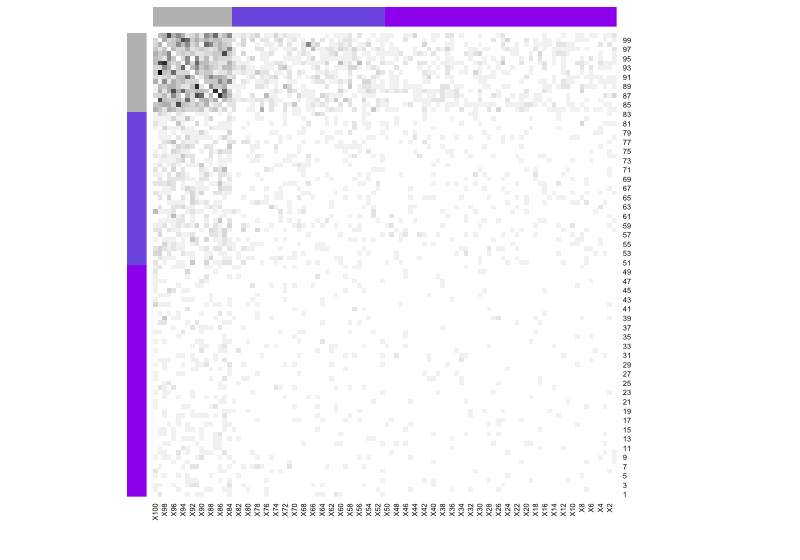
\includegraphics[width=.3333\textwidth,natwidth=800,natheight=560]{/Users/lapo_santi/Desktop/Nial/project/POMMs/power-law prior/Modular_code/WritingReport_plots/Adjacency_M4000.png}%
        \label{fig:M4000}%
    }\hfill
    \subfigure[M7000.png]{%
        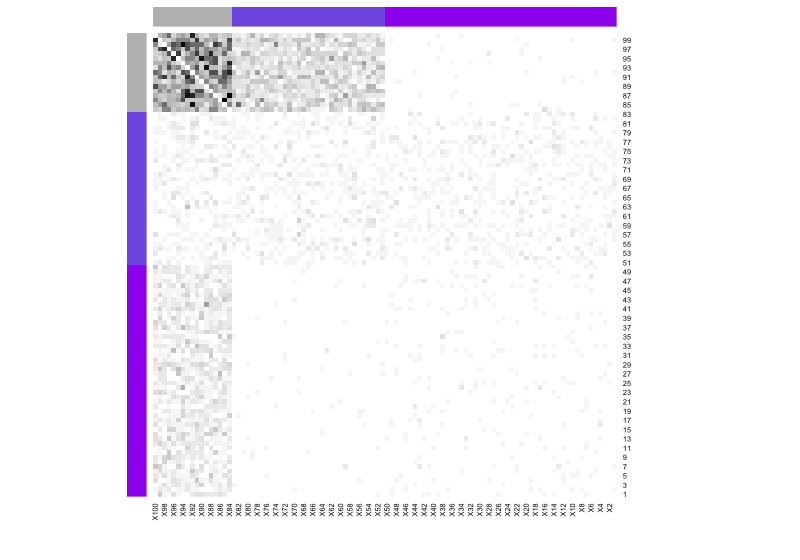
\includegraphics[width=.3333\textwidth,natwidth=800,natheight=560]{/Users/lapo_santi/Desktop/Nial/project/POMMs/power-law prior/Modular_code/WritingReport_plots/Adjacency_M7000.png}%
        \label{fig:M7000}%
    }\hfill
    \subfigure[M10000.png]{%
        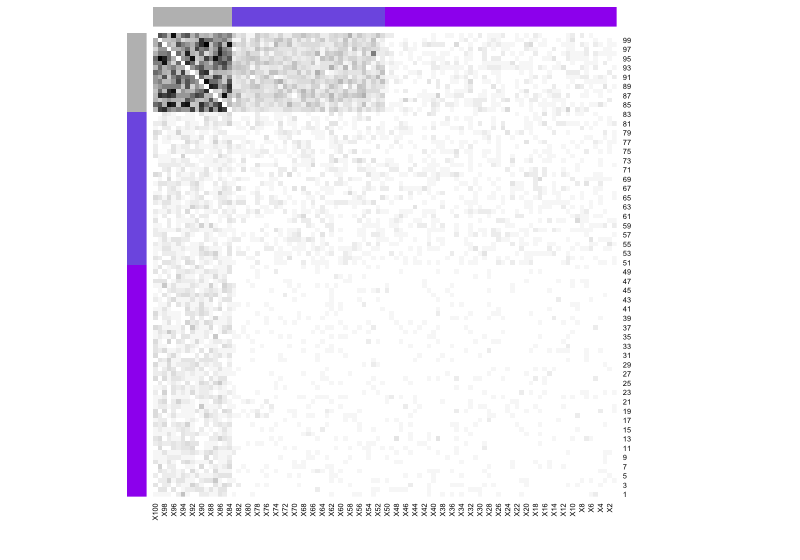
\includegraphics[width=.3333\textwidth,natwidth=800,natheight=560]{/Users/lapo_santi/Desktop/Nial/project/POMMs/power-law prior/Modular_code/WritingReport_plots/Adjacency_M_10000.png}%
        \label{fig:M10000}%
    }
    \caption{Images}
    \label{fig:all_images}
\end{figure}






\begin{table}[htbp]
\centering
\caption{$Y_{ij}$ drawn from a simple model}
\begin{tabular}{ccccccc}
\toprule
\multirow{2}{*}{Method} & \multicolumn{3}{c}{Macro Columns} & \multicolumn{3}{c}{Row Names} \\
\cmidrule{2-4} \cmidrule{5-7}
& $M=3000$ & $M=10000$ & $M=30000$ & Waic & VI distance & Predictive performance \\
\midrule
\multirow{3}{*}{Simple model} & - & - & - & - & - & - \\
& - & - & - & - & - & - \\
& - & - & - & - & - & - \\
\midrule
\multirow{3}{*}{POMM model} & - & - & - & - & - & - \\
& - & - & - & - & - & - \\
& - & - & - & - & - & - \\
\midrule
\multirow{3}{*}{Spectral Clustering} & - & - & - & - & - & - \\
& - & - & - & - & - & - \\
& - & - & - & - & - & - \\
\midrule
\multirow{3}{*}{K-means} & - & - & - & - & - & - \\
& - & - & - & - & - & - \\
& - & - & - & - & - & - \\
\midrule
\multirow{3}{*}{DBscan algorithm} & - & - & - & - & - & - \\
& - & - & - & - & - & - \\
& - & - & - & - & - & - \\
\bottomrule
\end{tabular}
\end{table}



\begin{table}[htbp]
\centering
\caption{$Y_{ij}$ drawn from a simple model}
\begin{tabular}{cccccc}
\toprule
\multirow{2}{*}{Method} & \multicolumn{4}{c}{Macro Columns} \\
\cmidrule{2-4}
&Measures& $M=3000$ & $M=10000$ & $M=30000$ \\
\midrule
\multirow{3}{*}{\shortstack{Simple \\ model}} & Waic & - & - & - \\
&VI distance & -& - & - \\
& Predictive performance & -& - & - \\
\midrule
\multirow{3}{*}{\shortstack{POMM \\ model}} & Waic& - & - & - \\
& VI distance& - & - & - \\
& Predictive performance & -& - & - \\
\midrule
\multirow{3}{*}{\shortstack{Spectral \\ Clustering}} & Waic & -& - & - \\
& VI distance& - & - & - \\
& Predictive performance& - & - & - \\
\midrule
\multirow{3}{*}{K-means} & Waic& - & - & - \\
& VI distance & -& - & - \\
& Predictive performance & -& - & - \\
\midrule
\multirow{3}{*}{DBscan algorithm} & Waic & -& - & - \\
& VI distance & -& - & - \\
& Predictive performance & -& - & - \\
\bottomrule
\end{tabular}
\end{table}













\begin{landscape}
\begin{table}[htbp]
\centering
\caption{$Y_{ij}$ drawn from a simple model}
\begin{tabular}{cccccccccc}
\toprule
\multirow{2}{*}{Method} & \multicolumn{3}{c}{$M=3000$} & \multicolumn{3}{c}{$M=10000$} & \multicolumn{3}{c}{$M=30000$} \\
\cmidrule(lr){2-4} \cmidrule(lr){5-7} \cmidrule(lr){8-10}
& Waic & VI distance & Pred. perf. & Waic & VI distance & Pred. perf. & Waic & VI distance & Pred. perf. \\
\midrule
Simple model & - & - & - & - & - & - & - & - & - \\
POMM model & - & - & - & - & - & - & - & - & - \\
Spectral Clustering & - & - & - & - & - & - & - & - & - \\
K-means & - & - & - & - & - & - & - & - & - \\
DBscan algorithm & - & - & - & - & - & - & - & - & - \\
\bottomrule
\end{tabular}
\end{table}
\end{landscape}


\begin{comment}

\section{Idea about a Gibbs sampler}

To derive the full conditional distribution of $\textbf{z}$ given the data $y$ and the hyperparameters $\boldsymbol{\gamma}$, we can use Bayes' theorem and write:

\begin{align*}
p(\textbf{z}|y,\boldsymbol{\gamma}) &\propto p(y|\textbf{z}) p(\textbf{z}|\boldsymbol{\gamma}) \
&\propto \prod_{i=1}^n \prod_{j=i+1}^n {n_{ij} \choose y_{ij}} (p_{z_i,z_j})^{y_{ij}} (1-p_{z_i,z_j})^{n_{ij}-y_{ij}} \prod_{k=1}^K \frac{\Gamma(\gamma_k + m_k)}{\Gamma(\gamma_k)}
\end{align*}

where we have dropped constant terms that do not depend on $\textbf{z}$. We can simplify this expression by collecting terms that depend on each $z_i$. Specifically, we can group the terms in the likelihood that involve $z_i$ with the prior probability of $z_i$ to get:

\begin{align*}
p(z_i|y,\textbf{z}{-i},\boldsymbol{\gamma}) &\propto p(y{i,\cdot}|\textbf{z}) p(z_i|\boldsymbol{\gamma}) \
&= \prod_{j\neq i} {n_{ij} \choose y_{ij}} (p_{z_i,z_j})^{y_{ij}} (1-p_{z_i,z_j})^{n_{ij}-y_{ij}} \frac{\Gamma(\gamma_{z_i} + m_{z_i})}{\Gamma(\gamma_{z_i})}
\end{align*}

where $\textbf{z}{-i}$ denotes all elements of $\textbf{z}$ except for $z_i$, and $y{i,\cdot}$ denotes the $i$th row of the $n\times n$ matrix of observations $y$. We can recognize the above expression as the likelihood of $z_i$ being drawn from a categorical distribution with parameter vector $\boldsymbol{\theta}{-i}$, where $\theta{k,-i} \propto \prod_{j\neq i} (p_{k,z_j})^{y_{ij}} (1-p_{k,z_j})^{n_{ij}-y_{ij}} \frac{\Gamma(\gamma_k + m_k)}{\Gamma(\gamma_k)}$ is the partial likelihood of $z_i$ being assigned value $k$, with $z_j$ for $j\neq i$ fixed to their current values. Thus, we have:

\begin{align*}
p(z_i=k|y,\textbf{z}{-i},\boldsymbol{\gamma}) &= \frac{\theta{k,-i}}{\sum_{k'} \theta_{k',-i}}
\end{align*}

for each possible value of $k$. This gives the full conditional distribution of $z_i$ given the data, the other $z_j$'s, and the hyperparameters.


\section{Possible applications}
The POMM model can have various applications in fields where pairwise comparisons are made. Some examples of applications are:
\begin{itemize}
\item Sports Analytics: The POMM model can be used to rank sports teams based on their pairwise comparison results. It can also be used to predict the probability of a team winning a match against another team.

\item Marketing: The POMM model can be used to rank products based on their pairwise comparison results in surveys. It can also be used to estimate the probability of a customer preferring one product over another.

\item Decision Making: The POMM model can be used to rank options based on their pairwise comparison results. It can also be used to estimate the probability of one option being preferred over another in a decision-making process.

\item Social Science: The POMM model can be used to study social preferences by asking individuals to compare two different options. For example, it can be used to understand people's preferences for different political candidates, policies, or social norms.

\item Biology: The POMM model can be used to study the relative fitness of different genotypes in evolutionary biology or the preferences of animals for different stimuli in behavioral ecology.
\end{itemize}
Overall, the POMM model can be applied in any field where pairwise comparisons are made and where the goal is to rank or estimate the probabilities of different options.



\begin{align}\log \left(\Pr(\mathbf{x}\mid n, \boldsymbol{\alpha})\right) &= \log\left(\frac{\Gamma\left(\alpha_0\right)\Gamma\left(n+1\right)}
{\Gamma\left(n+\alpha_0\right)}\prod_{k=1}^K\frac{\Gamma(x_{k}+\alpha_{k})}{\Gamma(\alpha_{k})\Gamma\left(x_{k}+1\right)}\right) \\
 &= \log\left(\Gamma\left(\alpha_0\right)\right) + \log\left(\Gamma\left(n+1\right)\right) - \log\left(\Gamma\left(n+\alpha_0\right)\right) \\ 
 & \qquad + \sum_{k=1}^K\left[\log\left(\Gamma(x_{k}+\alpha_{k})\right) - \log\left(\Gamma(\alpha_{k})\right) - \log\left(\Gamma\left(x_{k}+1\right)\right)\right] \end{align}

\end{comment}




\end{document}